\documentclass[serif,xcolor=pdftex,dvipsnames,table,hyperref={bookmarks=false,breaklinks}]{beamer}

%%%%%%%%%%%%%%%%
% Change the macros below to configure the title slides
% for your course.
\newcommand{\coursename}{COMPSCI 590N}
\newcommand{\instructor}{Roy J. Adams}
\newcommand{\university}{University of Massachusetts Amherst}
\newcommand{\department}{College of Information and Computer Sciences}
%%%%%%%%%%%%%%%%

\newcommand\HUGE{\@setfontsize\Huge{50}{60}}

\newcommand{\settitlecard}[2]{
  \title[\coursename  Lecture #1] 
    {\coursename \\ Lecture #1: #2}
     \author[\instructor]{\instructor}
     \institute[\university]{
     \department\\
     \university
   }
\date{}
}

\newcommand{\maketitlepage}{
  \begin{frame}
  \titlepage
  %\center{
    %If you use the slides unmodified, retain the attribution below
  %  \tiny{Slides by Roy J. Adams (rjadams@cs.umass.edu). 
    %If you modify the slides, please retain the alternate attribution below
    %\tiny{Based on slides by Roy J. Adams (rjadams@cs.umass.edu). \\    
  %  }                                              
  %}  
  \end{frame}
}

\AtBeginSection[]
{
  \begin{frame}<beamer>{Outline}
    \tableofcontents[currentsection,subsectionstyle=hide]
  \end{frame}
}


\newcommand{\cut}[1]{}

\newcommand{\iconbox}[4]{
  \only<#1-#2>{
    \begin{columns}[T]
      \column{0.5in}
           \includegraphics[width=0.5in]{#3}
       \column{3.7in}
            #4
    \end{columns}
    \medskip
    \medskip
    \medskip
  }
}

\mode<presentation>{
  \usepackage{../beamertheme589theme}
  \setbeamercovered{invisible}
}

\mode<handout>{
  \usepackage{../beamertheme589theme}
  \setbeamercovered{transparent}
}


\usepackage[english]{babel}
\usepackage[latin1]{inputenc}
\usepackage{times}
\usepackage[T1]{fontenc}
\usepackage{amsmath}
\usepackage{amssymb}
\usepackage[noend]{algorithmic}
\usepackage{algorithm}
\usepackage{listings}
\usepackage{tcolorbox}
\usepackage{xmpmulti}

\renewcommand\mathfamilydefault{\rmdefault}

\newcommand{\setA}{\mathcal{A}}
\newcommand{\setB}{\mathcal{B}}
\newcommand{\setS}{\mathcal{S}}
\newcommand{\setV}{\mathcal{V}}
\DeclareMathOperator*{\union}{\bigcup}
\DeclareMathOperator*{\intersection}{\bigcap}
\DeclareMathOperator*{\Val}{Val}
\newcommand{\mbf}[1]{{\mathbf{#1}}}
\DeclareMathOperator*{\argmax}{arg\,max}
\DeclareMathOperator*{\argmin}{arg\,min}
\DeclareMathOperator*{\sign}{sign}
\newcommand{\deriv}[2]{\frac{\partial{#1}}{\partial{#2}}}

\lstdefinestyle{custompython}{
  belowcaptionskip=1\baselineskip,
  breaklines=true,
  frame=single,
  xleftmargin=\parindent,
  language=Python,
  showstringspaces=false,
  basicstyle=\footnotesize\ttfamily,
  keywordstyle=\bfseries\color{green!40!black},
  commentstyle=\itshape\color{purple!40!black},
  identifierstyle=\color{blue},
  stringstyle=\color{orange},
}
\lstset{style=custompython}

\makeatletter
\renewcommand*\env@matrix[1][*\c@MaxMatrixCols c]{%
  \hskip -\arraycolsep
  \let\@ifnextchar\new@ifnextchar
  \array{#1}}
\makeatother

\newcommand\norm[1]{\left\lVert#1\right\rVert}


\settitlecard{1}{Python Basics}

\begin{document}

\maketitlepage

\section{Course Overview}
\subsection{Foo}

\begin{frame}[t]{What is Python?}
% TODO: pretify
Python is an interpreted programming language designed to be readable, compact, and scalable.
	
 \centering
 \vspace{.5in}
 
\includegraphics[width=1.5in]{{../Figures/Python-logo-notext.svg}.png}
\end{frame}

\begin{frame}[t]{Why use Python?}
Python has a number of features that make it particular well suited for research and numerical computing:

\pause
\begin{itemize} [<+->]
\item Clear, readable syntax
\item Interactive mode
\item Modular and portable
\item Automatic memory management
\item Flexible code time vs. run time tradeoff
\item A commonly used, well-documented set of numerical libraries
\end{itemize}

\end{frame}

\begin{frame}[t]{Course Goals}

The goal of this course is to give the students necessary programming and algorithmic knowledge to be able to write effective numerical programs in Python of the type used in CS 589, 585, etc. Topics we will cover include:

\pause
\begin{itemize} [<+->]
\item Basic programming concepts in Python.
\item How numbers are represented in a computer and how to work with them.
\item Algorithms underlying many basic numerical functions:
\begin{itemize}
	\item linear algebra
	\item probability
\end{itemize}
\item Documentation, testing, and debugging in Python.
\end{itemize}

\end{frame}

\begin{frame}[t]{Prerequisites}
\begin{itemize} [<+->]
\item The course has no formal prerequisites; however, an undergraduate level understanding of linear algebra and probability is expected. \textbf{No programming experience is expected.}
\item The course will be taught so that students can take it concurrently with other CICS data science courses.
\end{itemize}

\end{frame}

% \begin{frame}[t]{Logistics}
%
% Logistics and course details:
%
% \pause
% \begin{itemize}[<+->]
% \item Lectures: Tu/Th 5:30-6:15pm
% \item Instructor Office Hours: M 2:00-4:00pm, CS 207
% \item Course Website: \url{https://moodle.umass.edu/}
% \item Discussion Board: \url{https://piazza.com/umass/fall2016/cs590n/}
% \item Course e-Mail: rjadams@cs.umass.edu
% \item Course Policies: Refer to the syllabus on Moodle site.
%
% \end{itemize}
% \end{frame}

\begin{frame}[t,label=current]{Text Books}

We will use two main sources, both of which can be found online (see the course website for links):

\pause
\begin{itemize}[<+->]
\item \textit{Introduction to Python for Computational Science and Engineering}. Hans Fangohr.
\item \textit{The SciPy Lecture Notes}.
\end{itemize}

\onslide<+->{Readings will be posted to Moodle and are intended to be completed before class.}

\end{frame}

\begin{frame}[t]{Other Resources}
	
	There exist \textbf{many} excellent python resources that may be helpful supplements. A few are:
	
\pause
\begin{itemize}[<+->]
\item \textit{The Python Tutorial.} https://docs.python.org/3/tutorial/
\item \textit{Google's Python Class.} https://developers.google.com/edu/python/
\item \textit{Fast Lane to Python: A quick, sensible route to the joys of Python coding.} Norm Matloff. http://heather.cs.ucdavis.edu/~matloff/Python/PLN/FastLanePython.pdf
\end{itemize}

\end{frame}

% \begin{frame}[t]{Course Evaluation}
%
% The evaluation for the course will be based on assignments and quizzes.
%
% \begin{itemize}[<+->]
% \item Quizzes (6) 40\%
% \item Homework Assignments (6) 60\%
% \end{itemize}
%
% \onslide<+->{Both quizzes and assignments will be assigned and handed in through Moodle.}
%
% \end{frame}
%
% \begin{frame}[t]{Quizzes}
%
% \begin{itemize}[<+->]
% \item Quizzes will be administered weekly on Moodle.
% \item To be completed by Thursday (generally).
% \item Lowest quiz score dropped.
% \item These are not intended to take much time, but to be a warmup for the week's material.
% \end{itemize}
%
% \end{frame}
%
% \begin{frame}[t]{Assignments}
%
% \begin{itemize}[<+->]
% \item Assignments are to be done alone.
% \item Assignments will generally be assigned on Thursdays and due the following Tuesday.
% \item Late policy:
% \begin{itemize}[<+->]
% 	\item If you know of an excused absence, use the form on the Moodle page \textbf{before the due date} to notify me.
% 	\item Late assignments will receive a zero.
% 	\item Lowest score among \textbf{submitted} assignments will be dropped.
% 	\item If you do not submit an assignment, it will receive a zero and will be counted.
% \end{itemize}
% \end{itemize}
%
% \end{frame}

\section{Using Python}
\subsection{Foo}

\begin{frame}[t]{Getting Started}
	Software you will need for this class:
	\begin{itemize}[<+->]
		\item Python 3.5
		\begin{itemize}[<+->]
			\item Grading will be done in 3.5.
		\end{itemize}
		\item Python modules: NumPy, SciPy
		\item Jupyter (optional for in-class demos)
	\end{itemize}
	\pause
	Recommendation: \textbf{Anaconda} is a complete data science environment that ships with all of the above. (https://www.continuum.io/downloads)
\end{frame}

\begin{frame}[t,fragile]{The Read-Eval-Print Loop}
	Python is an interpreted language. This means Python programs are not compiled as a whole (like C/C++), but are read and compiled one line at a time. This process is sometimes called the \textbf{Read-Eval-Print Loop}.
	
\pause
	\begin{tcolorbox}
		\begin{verbatim}
			(1) Read
			(2) Interpret
			(3) Compile
			(4) Execute
			(5) Print
			(6) Repeat (1)-(5)
		\end{verbatim}
	\end{tcolorbox}

\pause	
This process is extremely flexible and powerful, but can be slow if you are not careful.

\end{frame}

\begin{frame}[t]{Interactive Python}
	\begin{itemize}[<+->]
	
		\item One of the most powerful Python features is \textbf{Interactive Mode}.
		\item Interactive mode allows a user enter lines of code, one at a time, directly into the interpreter.
	\end{itemize}
	\pause
	\center
	\Huge{DEMO}

\end{frame}

\begin{frame}[t,fragile]{Running a script}
	Most of what you write, however, will be written in code files sometimes called scripts.
	\pause
		\begin{tcolorbox}
			\begin{verbatim}
				$ python script.py
			\end{verbatim}
		\end{tcolorbox}
		
	\pause
	\center
	\Huge{DEMO}

\end{frame}

% \begin{frame}[t]{Python Environments}
%
% \end{frame}

\section{Python Basics}
\subsection{Foo}

\begin{frame}[t,fragile]{Variables and Assignment}

	\begin{itemize}[<+->]
		\item Variables are used to give names to values.
		\item Names are assigned using the assignment operator, "="
	\end{itemize}

	\pause
	\begin{verbatim}
			>>> x = 2
			>>> x
			2
	\end{verbatim}
	\pause
	\begin{verbatim}
			>>> x = "this is a string"
			>>> x
			"this is a string"
	\end{verbatim}
	\pause
	\begin{verbatim}
			>>> y = x
			>>> y
			"this is a string"
	\end{verbatim}

\end{frame}

\begin{frame}[t,fragile]{Basic Data Types}
	\begin{itemize}[<+->]
		\item Integers, \verb|x = 2|
		\item Floats (non-integers), \verb|x = 2.5|
		\item Bools (True or False), \verb|x = True|
	\end{itemize}
	\pause
	\begin{tcolorbox}
	\begin{verbatim}
		>>> x = 1
		>>> x
		1
		>>> y = float(x)
		>>> y
		1.0
		>>> z = bool(y)
		>>> z
		True
	\end{verbatim}
	\end{tcolorbox}
\end{frame}

\begin{frame}[t,fragile]{Math Operators}
	\begin{itemize}[<+->]
		\item Python support all standard math operators.
		\item Arithmetic: +, -, *, /
		\item Exponentiation: **
		\item Remainder (mod): \%
		\item Increment: +=, -=
	\end{itemize}
	\pause
	\begin{tcolorbox}
		\begin{verbatim}
		>>> 2.0 + 3.0
		5.0
		>>> 3.0**2.0
		9.0
		>>> 10.0 % 3.0
		1.0
		>>> x = 5
		>>> x += 3
		>>> x
		8
	\end{verbatim}
	\end{tcolorbox}
\end{frame}

\begin{frame}[t,fragile]{Mixing Types}
	\begin{itemize}[<+->]
		\item Python will automatically choose a type if you mix them.
	\end{itemize}
	\pause
	\begin{tcolorbox}
		\begin{verbatim}
		>>> 2 * 3
		6
		>>> 2.0 * 3.0
		6.0
		>>> 2.0 * 3
		6.0
	\end{verbatim}
	\end{tcolorbox}
\end{frame}

% \begin{frame}[t,fragile]{A First Numerical Problem - Integer Division}
% 	\begin{itemize}[<+->]
% 		\item What happens if we divide an integer by an integer (e.g \verb|3/2|)?
% 	\end{itemize}
% 	\pause
% 	\begin{tcolorbox}
% 		\begin{verbatim}
% 		>>> 3 / 2
% 		1
% 		>>> 3 / 2.0
% 		1.5
% 		>>> 3 / float(2)
% 		1.5
% 	\end{verbatim}
% 	\end{tcolorbox}
%
% \end{frame}

\begin{frame}[t,fragile]{Logical Operators}
	\begin{itemize}[<+->]
		\item Python also supports standard logical operators.
		\item Comparators: <, <=, ==, >=, >, !=
		\item Logical and/or: \verb|and|, \verb|or|
		\item Negation: \verb|not|
	\end{itemize}
	
	\pause
	\begin{tcolorbox}
		\begin{verbatim}
		>>> a = 2.0
		>>> b = 3.0
		>>> a > b
		False
		>>> not a > b
		True
		>>> (a > b) or (b == 3.0)
		True
	\end{verbatim}
	\end{tcolorbox}
\end{frame}

\begin{frame}[t,fragile]{Strings}
	\begin{itemize}[<+->]
		\item Strings store store text.
		\item Create strings using quotations: e.g. \verb|x = "this is a string"|
		\item Strings support many of the same operations as numeric types including: +, *, <, <=, ==, ...
	\end{itemize}

	\pause
	\begin{tcolorbox}
		\begin{verbatim}
			>>> "abc" + "de"
			'abcde'
			>>> 2*"abc"
			'abcabc'
			>>> "abc" == 'abc'
			True
			>>> "a" < "b"
			True
		\end{verbatim}
	\end{tcolorbox}

\end{frame}

\begin{frame}[t,fragile]{Lists and Tuples}
	\begin{itemize}[<+->]
		\item Lists and Tuples store sequences of objects.
		\item Contents can be mixed types.
	\end{itemize}

	\pause
	\begin{tcolorbox}
		\begin{verbatim}
			>>> a = [1,2,'a','b'] # Lists use []
			>>> a
			[1, 2, 'a', 'b']
			>>> b = (1,2,a,'string') # Tuples use ()
			>>> b
			(1, 2, [1, 2, 'a', 'b'], 'string')
			>>> len(b) # Length of a sequence
			4
		\end{verbatim}
	\end{tcolorbox}

\end{frame}

\begin{frame}[t,fragile]{Accessing sequences}
	\begin{itemize}[<+->]
		\item Individual entries of a List, Tuple, or String can be accessed using indexing.
		\item Access groups of elements using a ":".
	\end{itemize}

	\pause
	\begin{tcolorbox}
		\begin{verbatim}
			>>> a = [1,2,'a','b']
			>>> a[0] # Indexing is zero based
			1
			>>> a[2]
			'a'
			>>> a[1:4] # Returns positions 1 to 3
			[2,'a','b']
			>>> a[-1]
			'b'
		\end{verbatim}
	\end{tcolorbox}

\end{frame}

\begin{frame}[t,fragile]{Dictionaries}
	\begin{itemize}[<+->]
		\item Dictionaries store key/value pairs.
		\item Values are accessed using the keys.
		\item Created using \{\}.
	\end{itemize}

	\pause
	\begin{tcolorbox}
		\begin{verbatim}
			>>> a = {'one':1,'two':2,'three':3}
			>>> a['two']
			2
			>>> a.keys()
			['three', 'two', 'one']
			>>> a.values()
			[3, 2, 1]
			>>>
		\end{verbatim}
	\end{tcolorbox}
\end{frame}

\begin{frame}[t]{Variables as Names}
	\begin{itemize}[<+->]
		\item A Python variable can be though as a name for an object.
		\item Multiple names may refer to the same object.
	\end{itemize}
\end{frame}

\begin{frame}[t]{Variables as Names}
    \centering
    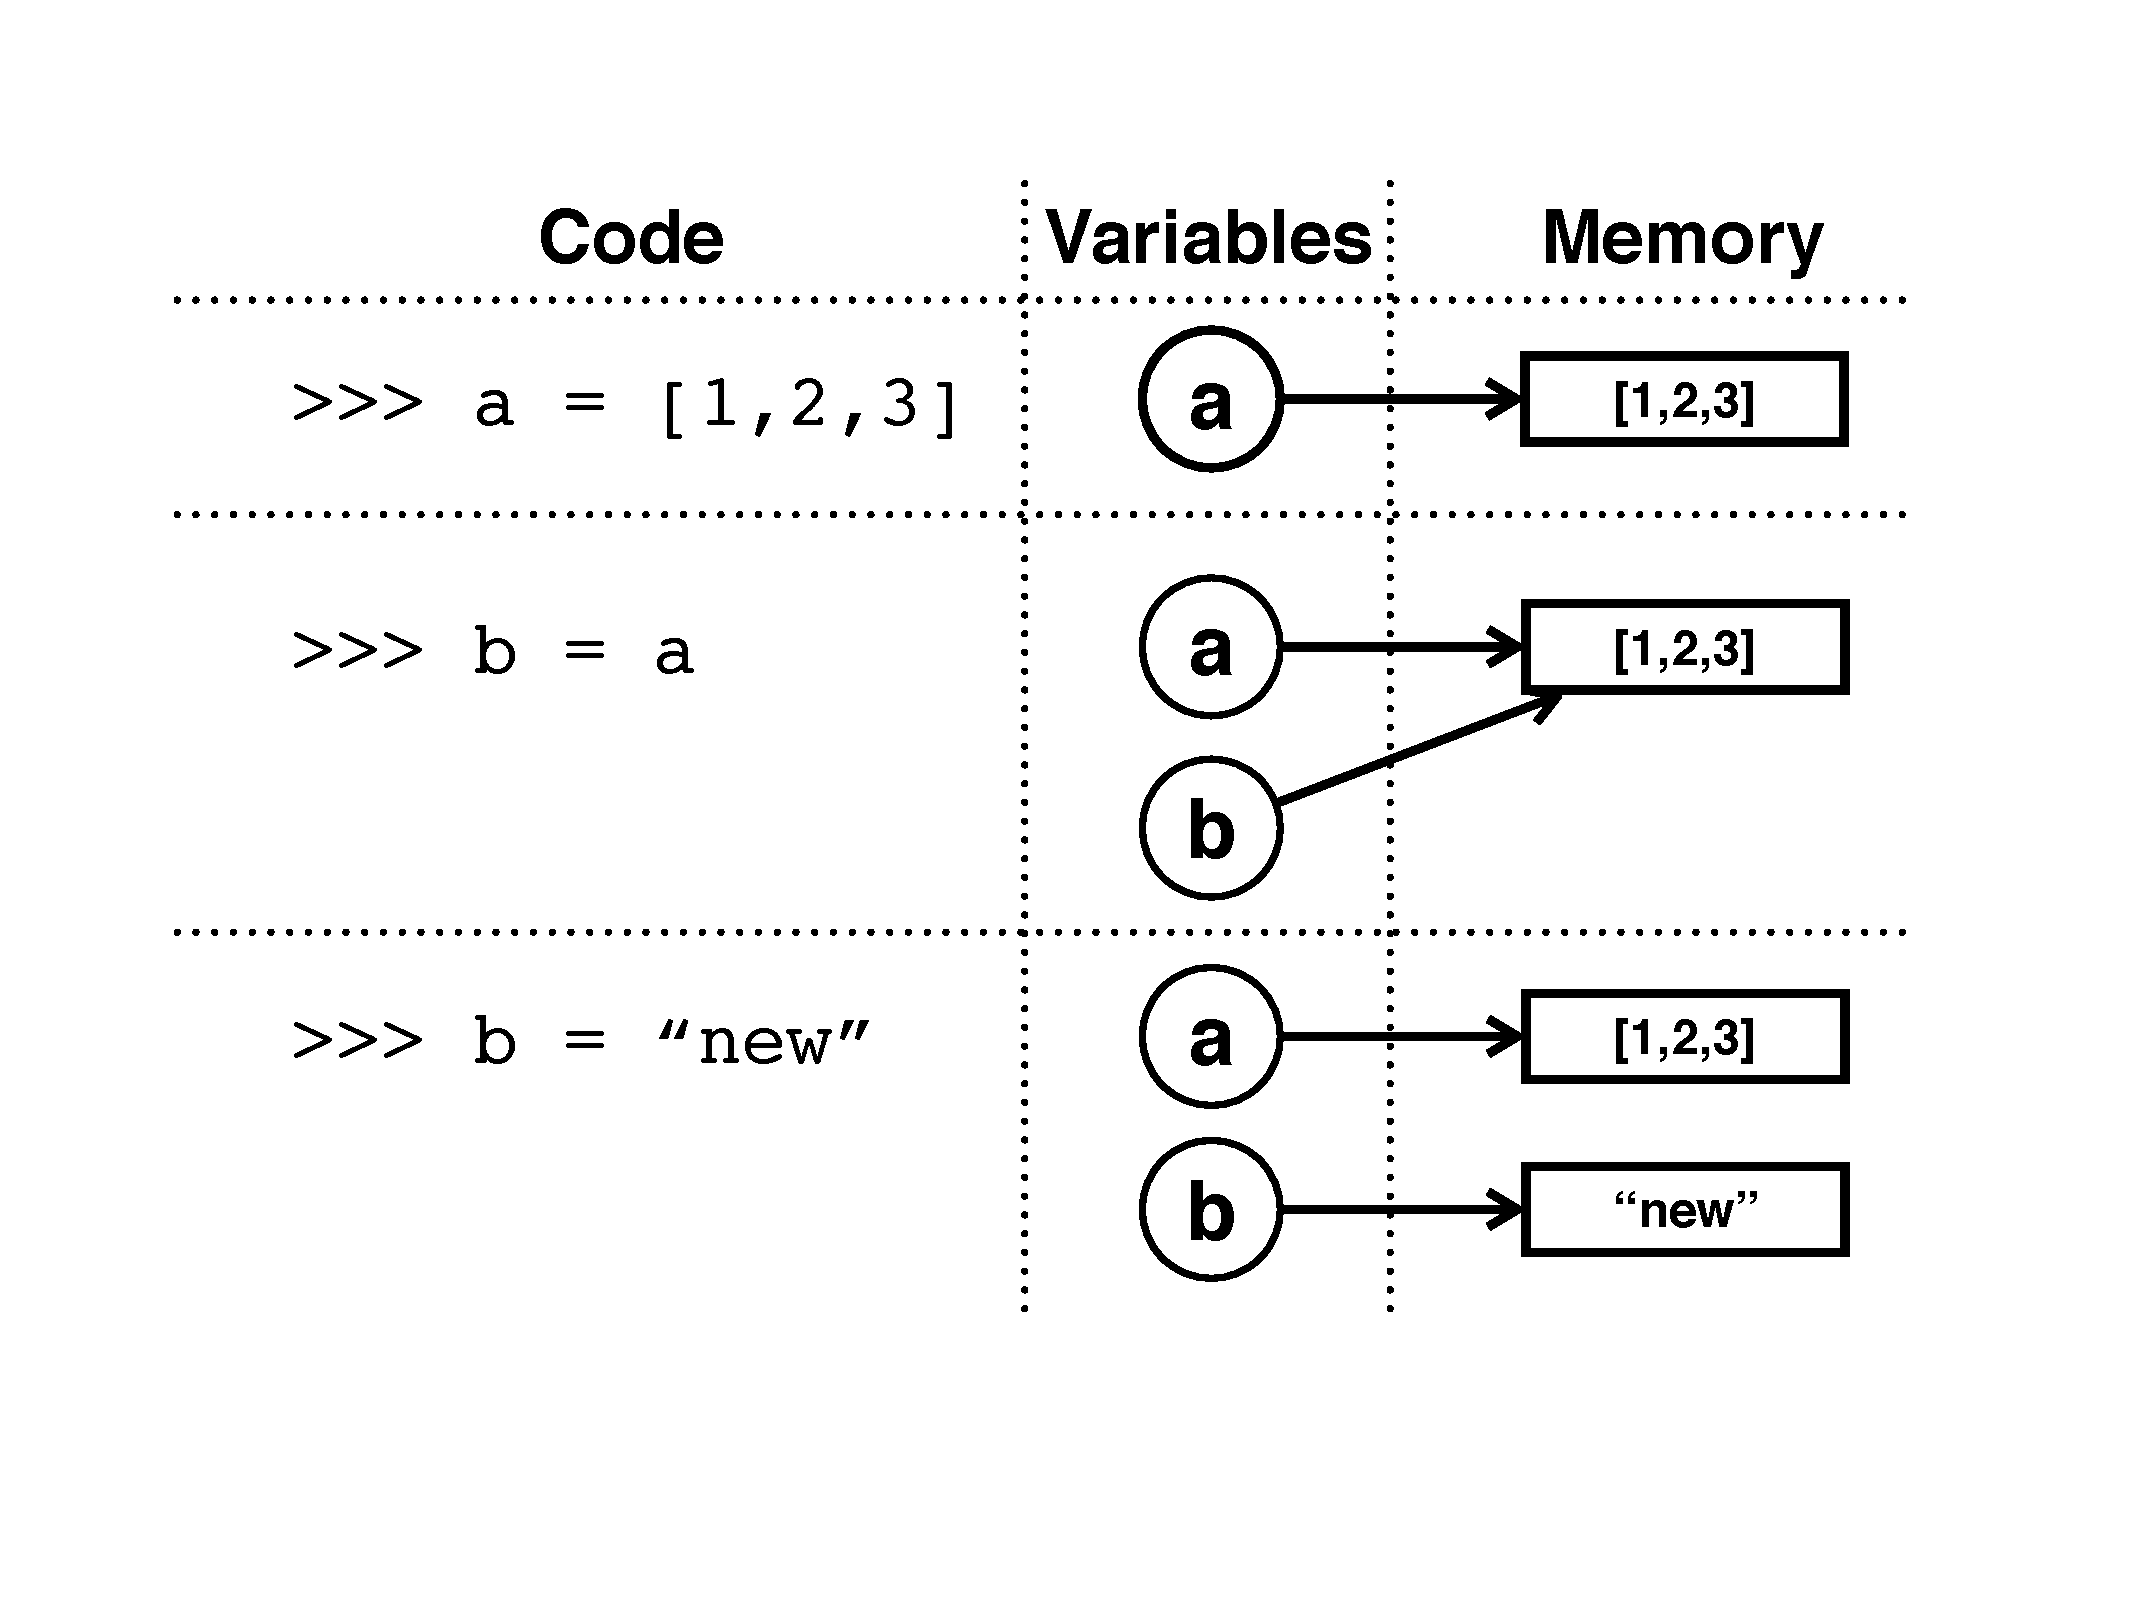
\includegraphics[width=4in]{{../Figures/variable_as_names}.pdf}
\end{frame}

\begin{frame}[t]{Variables as Names}
	\centering
	\Huge{DEMO}
\end{frame}

\begin{frame}[t]{Mutability}
	\begin{itemize}[<+->]
		\item A mutable object can have it's value changed. An immutable object cannot.
		\item Mutable: List, Dictionary
		\item Immutable: Int, Float, Bool, String, Tuple
	\end{itemize}

	\pause
	\centering
	\Huge{DEMO}
\end{frame}

% \begin{frame}[t,fragile]{Other Data Types}
% 	empty
% \end{frame}

\end{document}
